\documentclass[11pt]{article}

% basic packages
\usepackage[margin=1in]{geometry}
\usepackage[pdftex]{graphicx}
\usepackage{amsmath,amssymb,amsthm}
\usepackage{william}
\usepackage{tikz}
\usetikzlibrary{arrows.meta, positioning}

% page formatting
\usepackage{fancyhdr}
\pagestyle{fancy}

\renewcommand{\sectionmark}[1]{\markright{sf{\arabic{section}. #1}}}
\renewcommand{\subsectionmark}[1]{}
\lhead{bf{\thepage} \ \ \nouppercase{\rightmark}}
\chead{}
\rhead{}
\lfoot{}
\cfoot{}
\rfoot{}
\setlength{\headheight}{14pt}

\linespread{1.03} % give a little extra room
\setlength{\parindent}{0.2in} % reduce paragraph indent a bit
\setcounter{secnumdepth}{2} % no numbered subsubsections
\setcounter{tocdepth}{2} % no subsubsections in ToC

\begin{document}

% make title page
\thispagestyle{empty}
\bigskip \
\vspace{0.1cm}

\begin{center}
{\fontsize{22}{22} \selectfont Lecture Notes on}
\vskip 16pt
{\fontsize{36}{36} \selectfont \bf \sffamily Machine Learning}
\vskip 24pt
{\fontsize{18}{18} \selectfont \rmfamily Will Lancer} 
\vskip 6pt
{\fontsize{14}{14} \selectfont \ttfamily will.m.lancer@gmail.com} 
\vskip 24pt
\end{center}

{\parindent0pt \baselineskip=15.5pt}
\noin
Notes on machine learning.

% make table of contents
\newpage
\microtoc
\newpage

% main content
\section{Kaggle and Google's \emph{Introduction to Machine Learning}}

See the \href{https://github.com/will-lancer/notes/Computer_Science/Python/Python.pdf}{notes} 
on Python to refresh on the necessary NumPy and Pandas
to follow the example below.

\begin{iidea}
    [Basic terminology]
    Your data points are called
    \vocab{examples}, your parameters are called \vocab{features},
    and your desired prediction parameter is called the \vocab{label}.
    There are a few distinctions in machine learning:
    \begin{itemize}
        \item \vocab{Supervised learning} vs. \vocab{unsupervised learning}. Supervised
        just means you give the model the right answer in the end,
        and unsupervised means you don't (doing that may not even be well-defined).
        \item Supervised learning: \vocab{regression} vs. \vocab{categorization}.
        Regression predicts a numerical value and categorization predicts
        a likelihood that the label is in a given category. You can have binary
        or multi-category categorification.
        \item \vocab{Reinforcement learning} (broader than supervised/unsupervised).
        Gives the model rewards/punishments based on actions peformed within
        its training environment.
    \end{itemize}
    The basic ML workflow is
    \begin{center}
    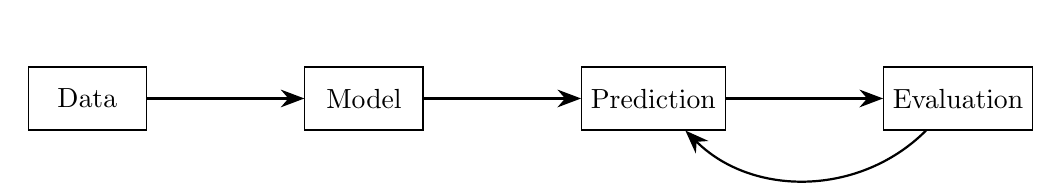
\begin{tikzpicture}[
        node distance=2cm,
        box/.style={rectangle, draw, minimum width=1.5cm, minimum height=0.8cm, align=center},
        arrow/.style={-{Stealth[length=3mm]}, thick}
    ]
        % Main flow nodes
        \node[box] (data) {Data};
        \node[box, right=of data] (model) {Model};
        \node[box, right=of model] (prediction) {Prediction};
        \node[box, right=of prediction] (evaluation) {Evaluation};
        
        % Main flow arrows
        \draw[arrow] (data) -- (model);
        \draw[arrow] (model) -- (prediction);
        \draw[arrow] (prediction) -- (evaluation);
        
        % Feedback loop arrow
        \draw[arrow] (evaluation) to[bend left=45] (prediction);
    \end{tikzpicture}
    \end{center}
    where your prediction and evaluation cycles continue ad infinitum.
\end{iidea}


\begin{eexample}
    [The decision tree]
    This extended example is Kaggle's intro course. It will help us get familiar
    with the general process before going into deeper theory.
    We first need to make our data into a DataTable to do analysis on it.
    We can import it from a csv by using \verb|df = pd.read_csv(dataFilePath)|.
    We look through our data using \verb|df.describe()| and \verb|df.head()|.
    We now need to specify featurese and a label. We do this by
    \begin{verbatim}
        features = ['column1', 'column2', ..., 'columnN']
        # 'X' is the standard name for the vector of feature data
        X = df[features]
        # 'y' is the standard name for the label vector
        y = df['labelColumn']
    \end{verbatim}
    Then we use some machine learning magic to train this data on this data set.
    For the decision tree, we import the decision tree trainer and then run it on the
    data,
    \begin{verbatim}
        from sklearn.tree import DecisionTreeRegressor
    \end{verbatim}
    We then declare a decision tree regression model and train it
    on our data,
    \begin{verbatim}
        decisionTree = DecisionTreeRegressor(random_state = 1)
        decisionTree.fit(X, y)
    \end{verbatim}
    Now we can use this to predict things, so we can say things
    like \verb|decisionTree.predict()| or \verb|decisionTree.predict(X.head())|
    to get predictions. You can optimize the number of leaves in your
    decision tree by minimizing the \vocab{mean absolute error},
    which is defined as
    \begin{align*}
        {\rm MAE} = \frac{1}{N} \sum_i^N |\mathbf{y}_{\rm train} - \mathbf{y}_{\rm val}|.
    \end{align*}
    You can import the mean absolute error module from \verb|sklearn.metrics|
    like before,\\ \verb|import mean_absolute_error|.
    You can also import a train-test-split tool from\\
    \verb|sklearn.model_selection|
    to get some validation data from your training set.
\end{eexample}

That's it! That's our first basic ML model.






\end{document}